% #################################################
% Inhalt 
% #################################################
%\include{Inhalt/01_Einleitung}
%\include{Inhalt/content}



\chapter{Einleitung}
\section{Erster Untergliederungspunkt}
\blindtext

\chapter{Das zweite Kapitel}
\blindtext

\chapter{Formatierung von Grafiken und Tabellen}
Grafiken, Bilder und Tabellen sind wichtige Bestandteile einer wissenschaftlichen Arbeit. Dieser Abschnitt zeigt Ihnen die wichtigsten Grundregeln für eine Arbeit auf. 


\section{Einbinden von Grafiken}
Alle Abbildungen der Arbeit sollten an mindestens einer Stelle im Fließtext auch referenziert werden. 


Abbildung~\ref{fig:example} zeigt beispielhaft eine Abbildung in einer Abschlussarbeit. Jede Abbildung muss zwingend auch eine Bildunterschrift haben. Diese kann knapp ausfallen, aber auch ausführlich als Ergänzung zum Fließtext gehalten werden. Das Code-Beispiel~\ref{lst:images} zeigt, wie Sie Bilder in Latex einbinden können. 
\begin{figure}
\centering
  \label{fig:example}
  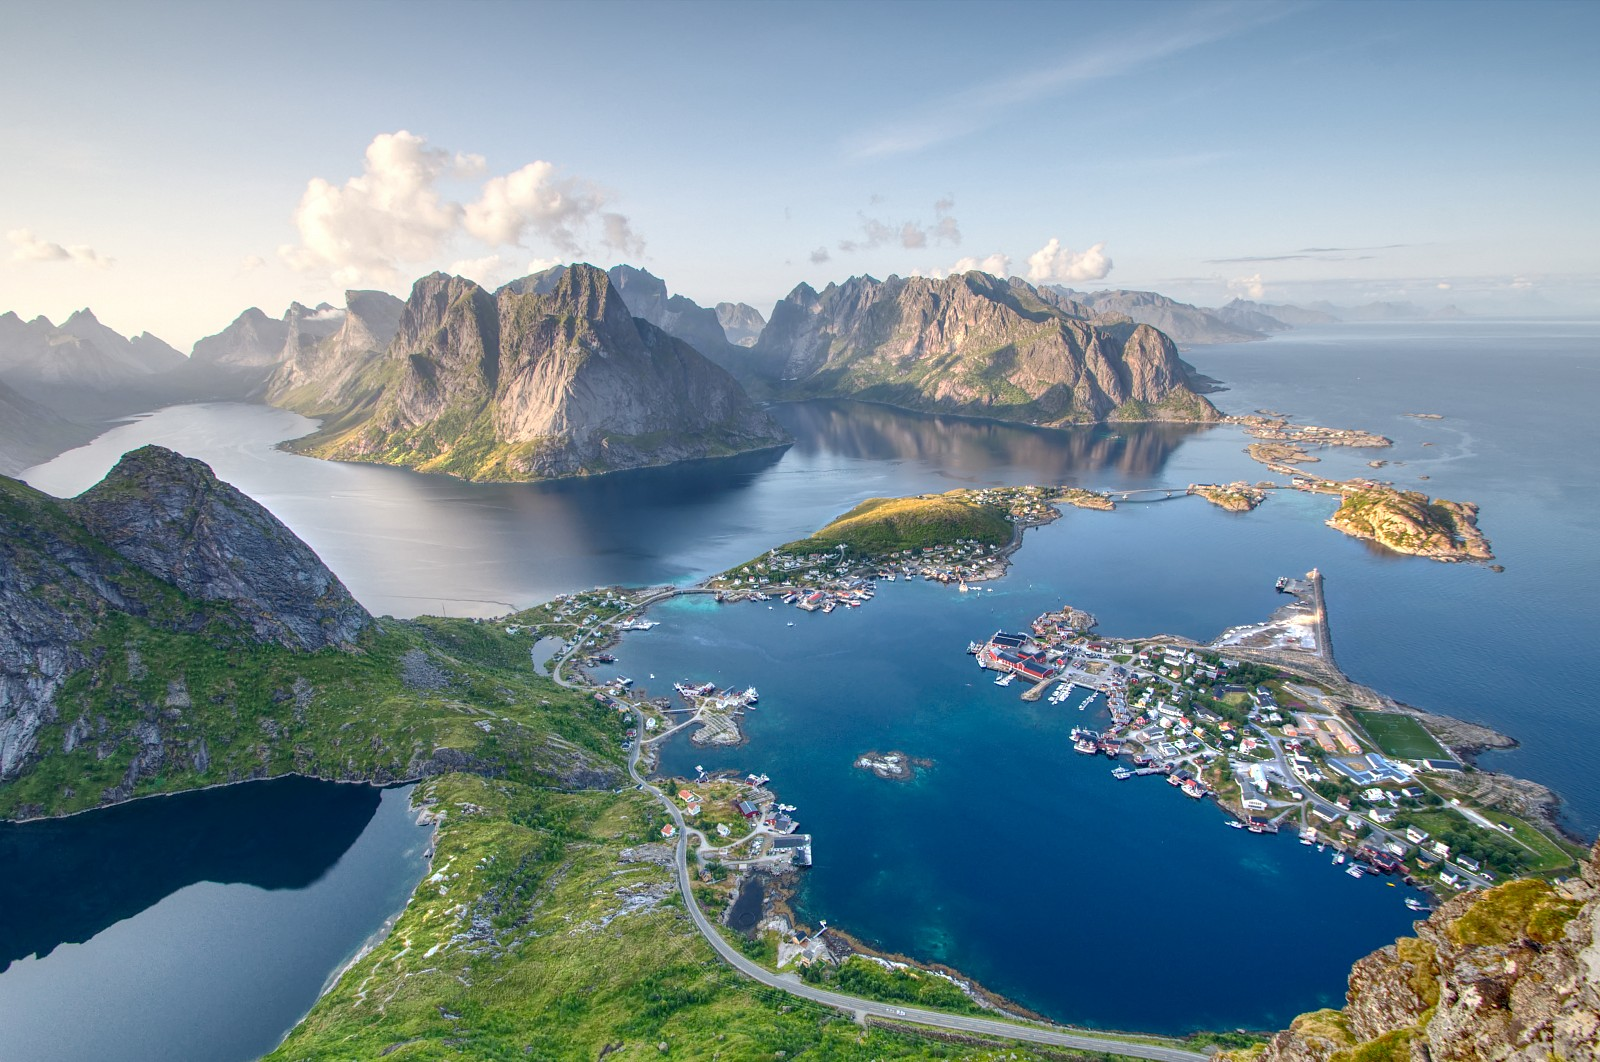
\includegraphics[width=0.4\textwidth]{02_images/example_image_1}
  \caption{Das ist eine Beispielgrafik. Quelle: Christian Pfitzner }
\end{figure}

Bilder können auch platzsparend nebeneinander formatiert werden. 
\begin{figure}
\label{lst:images}

\begin{lstlisting}[caption={Codebeispiel zum Einbinden von Bildern \label{fig:example}}]
\begin{figure}
\centering
  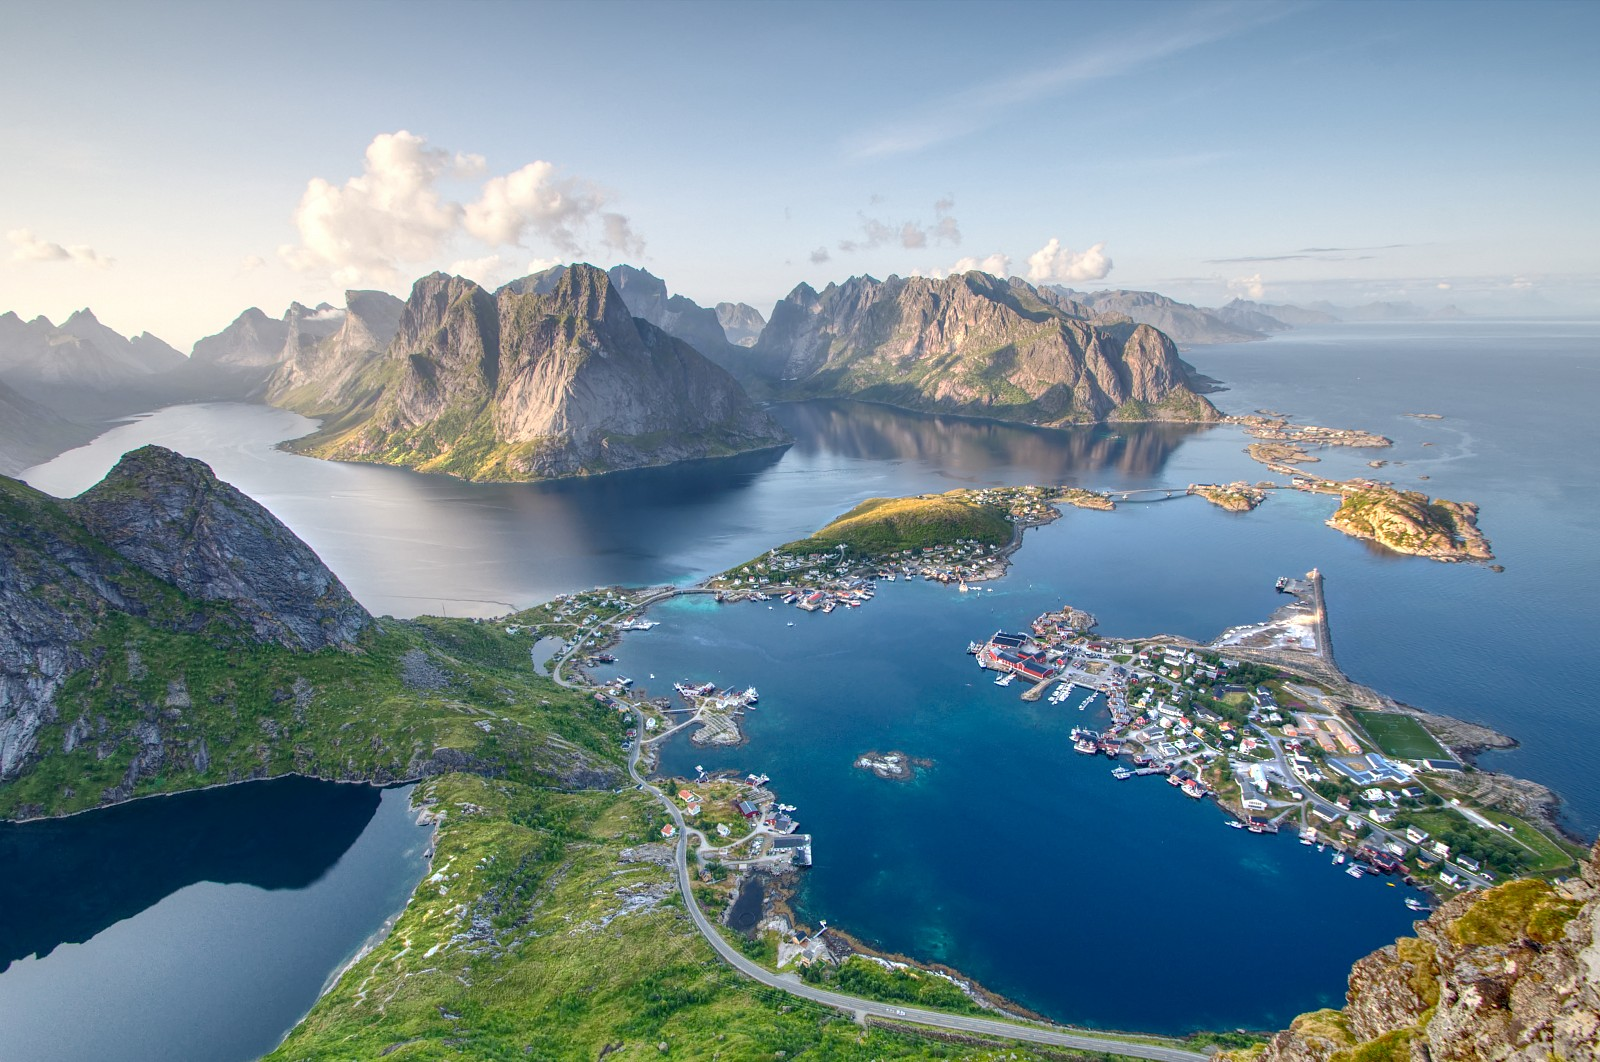
\includegraphics[width=0.4\textwidth]{02_images/example_image_1}
  \caption{Das ist eine Beispielgrafik. Quelle: Christian Pfitzner }
\end{figure}
\end{lstlisting}
\end{figure}



Tabelle~\ref{tab:example} zeigt beispielhaft eine Tabelle inklusive Tabellenüberschrift. 
\begin{table}
\label{tab:example}
\centering
\caption{Das ist eine Beispieltabelle mit Tabellenüberschrift. }
\begin{tabular}{lll}
\toprule
\textbf{Überschrift 1}& \textbf{Überschrift 2} & \textbf{Überschrift 3} \\
\midrule
Ein Element   & Noch ein Element & Noch ein Element \\
1 & 2 & 3\\
\bottomrule
\end{tabular}
\end{table}






%\nocite{*}
\bibliographystyle{plain} 
%\inputencoding{latin2}
\bibliography{references}
%\inputencoding{utf8}

% #################################################
% Anhang 
% #################################################
\begin{appendix}
    \clearpage    
    \pagenumbering{roman}
    \setdefaultleftmargin{1em}{}{}{}{}{}     
    %\input{Anhang}
\end{appendix}